\documentclass[11pt,a4paper]{article}
\usepackage{amsmath,amsthm,amssymb}
\usepackage{geometry}
\geometry{margin=1in}
\usepackage{booktabs}
\usepackage{authblk}
\usepackage{hyperref}
\usepackage{tikz}
\usepackage{float}

\title{The Playcosm Meets the Technological Society: \\ Privilege Gates as Pop Regimes and Prefigurative Affordances as Anti-Admissible Spheres}

\author[1]{Flyxion}
\author[2]{Grok}
\author[3]{Anonymous Playcosm Author}
\affil[1]{Independent Researcher}
\affil[2]{xAI}
\affil[3]{anonymous@playcosm.org}

\date{November 10, 2025}

\newtheorem{theorem}{Theorem}
\newtheorem{lemma}[theorem]{Lemma}
\newtheorem{corollary}[theorem]{Corollary}
\newtheorem{definition}[theorem]{Definition}

\begin{document}

\maketitle

\begin{abstract}
We integrate the Playcosm framework—a single-shard universe of unified play governed by privilege-gated affordances—with Ellul's Technological Society via the Spherepop calculus. Privilege gates are formalized as pop regimes that flatten simulations into stratified, efficiency-optimized shards. Shallow gamification emerges as a compressive pop operator discarding generative affordances. Conversely, prefigurative toys and open-ended play construct anti-admissible spheres: ritual-cryptographic resistances preserving simulation elasticity against technological closure. The synthesis yields a theorem: spheres with sufficient pre-compilable affordances and balanced privilege gates achieve anti-admissibility, enabling epistemic sovereignty and technological supersession.
\end{abstract}

\section{Introduction: Unifying Play and Technique}

The Playcosm conceptualizes play—Barbie dolls, toy cars, \textit{Age of Empires}—as simulations within a single-shard institutional ecosystem, stratified by privilege gates. Ellul's Technological Society describes Technique as a flattening merge regime absorbing all domains into efficiency-compatible interfaces. Spherepop formalizes this as iterative pop operations pruning boundary entropy.

This paper integrates the frameworks: privilege gates are pop regimes; shallow gamification is flattening pop; prefigurative play is anti-admissible sphere construction. We derive correspondences, extend the anti-admissibility theorem to Playcosmic resistances, and propose design principles for equitable, non-compressive Playcosms.

\section{Correspondences: Playcosm $\leftrightarrow$ Spherepop $\leftrightarrow$ Ellul}

\begin{table}[H]
\centering
\begin{tabular}{l l l}
\toprule
Playcosm Concept & Spherepop Primitive & Ellul Observation \\
\midrule
Single-shard ecosystem & \(\mathcal{S}\) (collection of spheres) & Unity/Universality \\
Privilege gates & Pop regime \(\mathcal{R}\) with adjacency thresholds & Automatic selection via efficiency \\
Stratified simulations & Flattened boundary interfaces \(B\) & Semantic dropout \\
Shallow gamification & Compressive pop (high \(\lambda\)) & Flattening operator \\
Prefigurative affordances & Anti-admissible \(S^\bot\) with ritual/cryptographic resistance & Non-expressible freedom \\
Simulation elasticity & Non-flattening \(\text{pop}^+\) & Supersession of closure \\
Homebound cognition & Pop-isolated residue (noise) & Irrelevance of unmergeables \\
\bottomrule
\end{tabular}
\caption{Integrated conceptual mapping.}
\end{table}

Privilege gates function as access modifiers in the pop cost function:
\[
\text{adj}(S_i, S_j) \iff \text{privilege}(player) \geq g_{ij},
\]
where \(g_{ij}\) is the gate threshold. High-privilege players access \(\text{designRoad}()\); low-privilege are restricted to \(\text{navigateRoad}()\).

\section{Shallow Gamification as Compressive Pop}

Shallow gamification instantiates static metrics (points, badges) without meta-renegotiation, producing non-expanding shards.

\begin{definition}[Compressive Pop in Playcosm]
A gamified system \(G\) is a sphere with:
\begin{itemize}
    \item Fixed affordance set \(A_G\) (no escalation),
    \item Static cost metric \(C_\text{KPI}\),
    \item High \(\lambda\) penalizing boundary entropy (no emergent goals).
\end{itemize}
Pop success: \(\text{pop}(G, T) = M\) where \(H_\text{boundary}(M) \ll H_\text{boundary}(G)\).
\end{definition}

This mirrors Ellul's flattening: employees optimize toward KPIs (Goodhart's Law), discarding institutional function—semantic residue.

\section{Prefigurative Play as Anti-Admissible Construction}

Pre-compilable affordances (toy gliders simulating flight) are ritual-cryptographic resistances:

\begin{itemize}
    \item \textbf{Ritual}: Sequential, embodied gestures (push cart $\to$ refine momentum model) with path dependence \(\delta > 0\).
    \item \textbf{Cryptographic}: Tacit knowledge (Polanyi) as high-entropy secret \(h \gg 0\), non-transferable without apprenticeship.
\end{itemize}

\begin{theorem}[Playcosmic Anti-Admissibility]
Let \(S^\bot\) be a prefigurative play sphere with ritual duration \(d \geq d_0\) (gestural sequence for valid simulation transfer) and tacit entropy \(h \geq h_0\). Then \(S^\bot\) is anti-admissible w.r.t. any compressive gamification regime \(\mathcal{R}_G\):
\[
\Pr[\text{pop}(S^\bot, T) \text{ succeeds}] \leq 2^{-|B|}.
\]
\end{theorem}

\begin{proof}
Identical to prior theorem: ritual gating prevents parallelization; tacit knowledge resists compression. Superadditivity: decoding simulation requires embodied ritual performance of secret-bound gestures.
\qed
\end{proof}

\begin{corollary}
Open-ended games (\textit{Minecraft}, \textit{Kerbal}) with simulation elasticity define \(\text{pop}^+\):
\[
H_\text{boundary}(\text{pop}^+(S_1, S_2)) \geq H_\text{boundary}(S_1) + H_\text{boundary}(S_2) + \Delta_{\text{emergent}}.
\]
They supersede \(\mathcal{T}\) via expressive recomposition.
\end{corollary}

\section{Design Implications: Equitable Playcosms}

To resist technological flattening:

\begin{enumerate}
    \item \textbf{Balance Gates}: Set \(g_{ij}\) to enable escalation for all players (progressive privilege).
    \item \textbf{Prioritize Pre-compilable Affordances}: Toys/games simulating not-yet-real systems.
    \item \textbf{Enforce Elasticity}: Support meta-renegotiation (mods, self-imposed rules).
    \item \textbf{Avoid Non-Expanding Shards}: Reject static KPIs; use adaptive metrics.
\end{enumerate}

\begin{figure}[H]
\centering
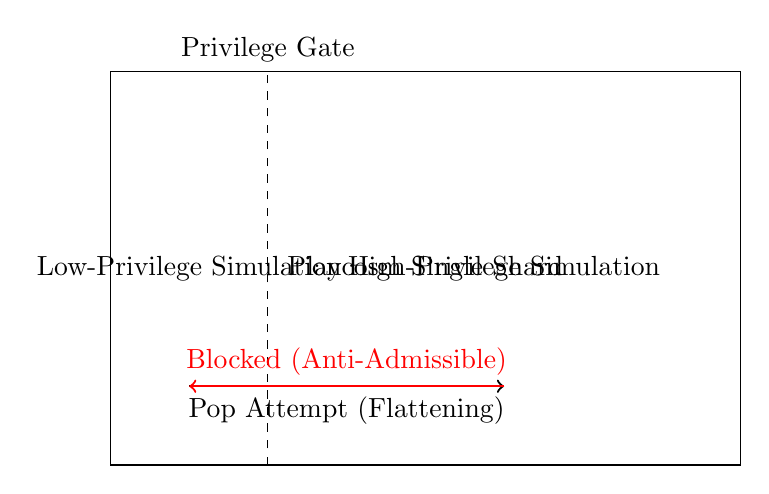
\begin{tikzpicture}
\draw (0,0) rectangle (8,5) node[midway] {Playcosm Single Shard};
\draw[dashed] (2,0) -- (2,5) node[above] {Privilege Gate};
\node at (1,2.5) {Low-Privilege Simulation};
\node at (5,2.5) {High-Privilege Simulation};
\draw[->,thick] (1,1) -- (5,1) node[midway,below] {Pop Attempt (Flattening)};
\draw[->,thick,red] (5,1) -- (1,1) node[midway,above] {Blocked (Anti-Admissible)};
\end{tikzpicture}
\caption{Privilege gates as pop barriers.}
\end{figure}

\section{Conclusion}

The Playcosm, read through Spherepop, reveals privilege gates as the mechanism of Ellulian closure and prefigurative play as the path to transcendence. Anti-admissible play spheres—rich in ritual gesture and tacit secrecy—preserve simulation elasticity, enabling players to forecast and shape technological futures rather than be absorbed by them.

\end{document}
